\chapter{Results}

\section{Deuteron photodisintegraion}

    \subsection{Cross section}
    In this section I will show the results of my calculation starting from the
    deuteron photodisintegration process. One of the most
    studying observable is obviously cross section. There is
    a number of papers which present 
    measurement results for both differential and total cross section
    \cite{BOSMAN1979,ARENDS1984,Skopik1974, Moreh1989, Birenbaum1985, Bernabei1986, rachek2007,Ying_Experiment_Deut, DeSanctis_Experiment_Deut} so it is convenient 
    to prepare a theoretical predictions in order to compare 
    it with experimental results.

    On the Fig.~\ref{TOTAL_CROSS} and Fig.~\ref{TOTAL_CROSS_small} 
    I present predictions for the
    total cross section $\sigma_{tot}~[\mu\text{b}]$ which I obtained
    using the chiral potential at the order N$^4$LO+ and with 
    the cut off parameter $\Lambda=450$~MeV (my best predictions).
    Looking at Fig.~\ref{TOTAL_CROSS_small}, we can see that at low photon energies
    (below 50 MeV) my predictions which include 2N contributions
    using Siegert approach, describe experimental results quite well.
    We can suppose that the difference with experimental data may come from 
    the statistical uncertainty of  the data itself, as my predictions
    are often in between the data from different sources.
    Moreover even at such low energies the 1N current is clearly not enough
    to describe this observable as dashed pink line has much lower values and
    the difference becomes even larger with larger photon's energies. 

    Having look at the higher energies (above 50~MeV, Fig.~\ref{TOTAL_CROSS})
    we can notice that the difference with experimental data is not only 
    quantitative, but also qualitative.  There is a peak around 300~MeV
    in the experimental data from \cite{Bernabei1986} which is not
    reflected in my predictions. The reason of such discrepancy 
    is most likely coming from the relativistic effects
    which I do not take into account. At higher energies their contribution
    becomes larger and here we observe a clear justification of such a lack.
    It is also confirmed by the calculations in \cite{ArenhovelPhotodisint1991}
    where authors present predictions obtained with and without including
    relativistic effects and such a peak appears in the latter case. 
    
    Nevertheless my main goal is to describe deuteron photodisintegration at low energies and predictions seem to be well describing experimental data at
    $E_\gamma \lesssim 50$~MeV. The higher energies region is presented in order
    to investigate how far the predictions are from experimental results and 
    what can be improved in the future (e.g. include relativistic part). 

    
    \begin{figure}[h]
        \begin{center}
        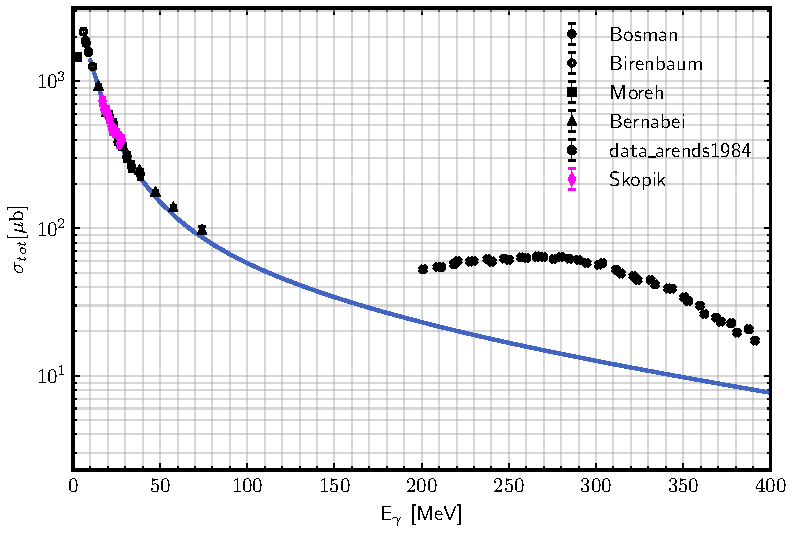
\includegraphics[width=0.75\textwidth]{Figures_python/TOTAL_CROSSSECTION.pdf}
        \end{center}
        \caption{Total cross section as a function of the photon's energy E$_\gamma$.
        Solid blue line presents results obtained with SN+Siegert 
        and dashed pink line - with only SN current.
        The experimental data are from \cite{Bernabei1986} (black filled circles),
        \cite{BOSMAN1979} (empty circles),
        \cite{ARENDS1984} (squares),
        \cite{Skopik1974} (triangles),
        \cite{Moreh1989} (cross "X") and
        \cite{Birenbaum1985} (dimonds).
        }
        \label{TOTAL_CROSS}
    \end{figure}
    

    \begin{figure}[h]
        \begin{center}
        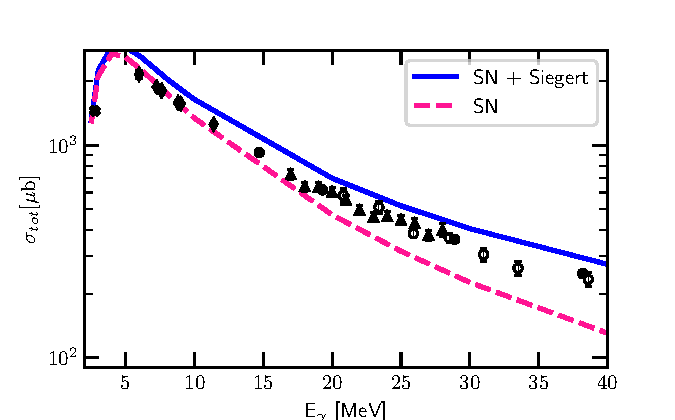
\includegraphics[width=0.75\textwidth]{Figures_python/TOTAL_CROSSSECTION_SMALL_REGION.pdf}
        \end{center}
        \caption{The same as on the Fig.~\ref{TOTAL_CROSS} but for the energy range 2.5 - 40 MeV.
        }
        \label{TOTAL_CROSS_small}
    \end{figure}
        
    {\color{red} Maybe better reorganize figures, combine similar figures for different energies in one?}

    Figures \ref{CROSS_30} - \ref{CROSS_140} show my predictions for the differential cross section
    $\frac{d\sigma}{d\Omega}$ at three values of the photon energy:
    30, 100 and 140~MeV. They all are organized in a similar way: the left panel
    presents predictions obtained using SMS potential at different chiral orders (from LO to N$^4$LO+)
    with cut off parameter $L = 450$~MeV,
    the middle panel includes the truncation error's bands (described in Sec. \ref{sec:deut_bound})
    for each chiral order starting
    from NLO. And the right panel shows predictions obtained with different values of the
    cut off parameter at the chiral order N$^4$LO+.

    Comparing the best predictions (N$^4$LO+, $\Lambda=450$~MeV) for each
    of the Fig.~\ref{CROSS_30} - \ref{CROSS_140} we can once more 
    conclude that the higher photon's energy is, the larger is 
    difference between the theoretical predictions and experimental 
    measurements. At $E_\gamma = 30$~MeV (Fig.~\ref{CROSS_30}) my predictions
    almost perfectly match the data and the difference is almost always
    within the experimental uncertainties. Going to the energy 100~MeV (Fig.~\ref{CROSS_100})
    the descriptions seems not to be such good: theoretical
    predictions match experimental data qualitatively, but
    the gap in the angles range ($60^{\circ} < \theta_p < 130^{\circ}$) 
    is around 30\% ({\color{red} check the value!}).
    Looking at the Fig.~\ref{CROSS_140} it is hard to say even about 
    good qualitative description, the general trend of the
    angular dependance is presented, but still the predictions are 
    far from experimental values.
    In addition, figures for each energy confirm the convergence 
    of the predictions with respect to the chiral order.
    We see that the curves at LO are far from both experimental 
    data and the best potential's predictions (N$^4$LO+) and
    the higher is photon's energy, the larger is this
    difference. With each subsequent chiral order, the 
    curves are more closer to each other and the difference
    between N$^4$LO and N$^4$LO+ is hardly visible at current scale.
    So I can conclude that predictions are converged and 
    further chiral orders would rather not bring large contribution 
    to the cross section values. What may be helpful
    in a better data description is a 2N current 
    and relativistic correction, mentioned earlier.

    The middle pane of Fig.~\ref{CROSS_30} - \ref{CROSS_140} 
    presents theoretical (truncation) uncertainties and it once more
    confirm that for the regarded nuclear reaction chiral order
    N$^4$LO+ is able to produce converged predictions: 
    the black band is hardly visible for the $E_\gamma=30$~MeV 
    and quit thin for larger energies. 
    The difference with experimental data is rather systematic 
    and is independent on the chiral order. 

    The right panes in discussed figures present a cut off dependency
    of my predictions. The ideal case is when the dependency is so weak that
    the choice of the parameter $\Lambda$ would not make large 
    changes. In practice the choice of this parameter can be 
    important as it makes a noticeable difference in predictions.
    
    On the Fig.~\ref{CROSS_30} the cut off dependance is so weak,
    that, in fact, all the lines (for different $\Lambda$ values)
    overlap each other and we cannot differentiate them with the naked eye.
    Nevertheless, with increasing photon's energy to 100 and 140~MeV (Fig.~\ref{CROSS_100}
    and Fig.~\ref{CROSS_140}) the spread becomes larger. 
    Although the spread is visible, it is not so large and even for 140~MeV
    it is within 12\%. 
    

    \begin{figure}[h]
        \begin{center}
        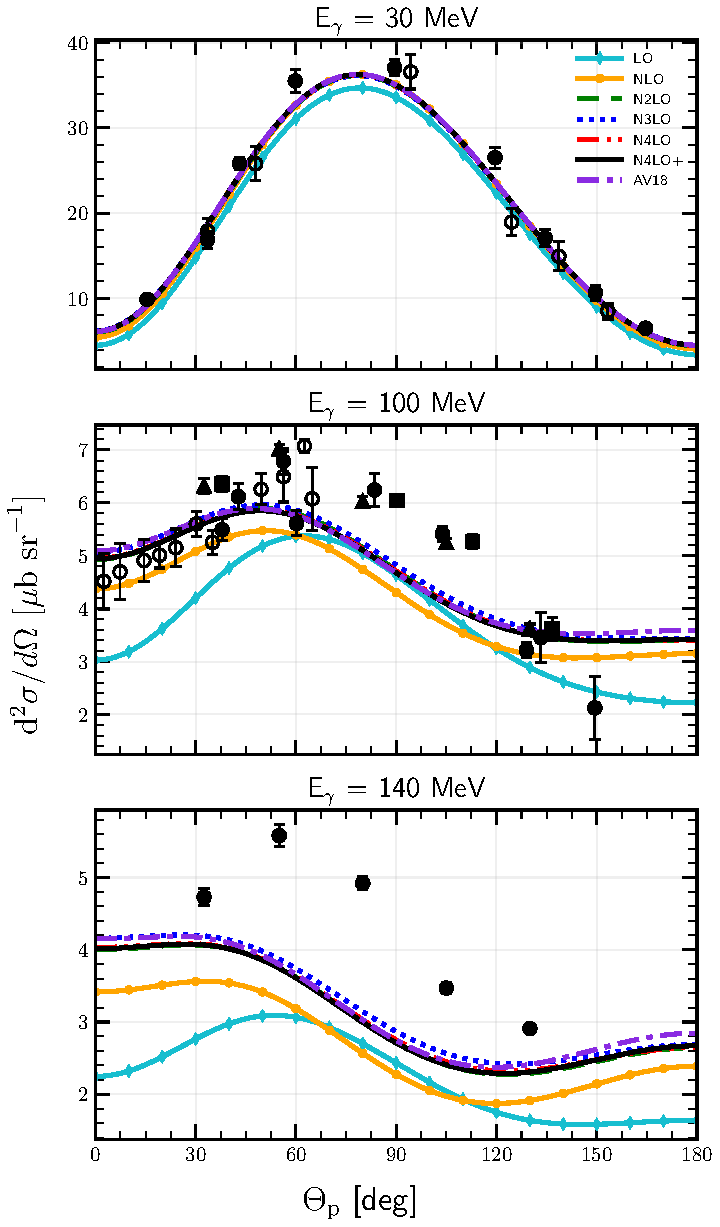
\includegraphics[width=0.7\textwidth]{Figures_python/CROSS2_order_vert.pdf}
        \end{center}
        \caption{Differential cross section as a function of the outgoing proton angle in the center of mass frame 
        for the photon's energy 30 MeV (top), 100 MeV (middle) and 140 MeV (bottom). Results are obtained using potential
        with different chiral orders (from LO to N$^4$LO+) with cutoff parameter $\Lambda=450$~MeV.
        For the sake of comparison, predictions obtained with AV18 potential are on both figures as well.
        Data points (filled and empty circles) are from \cite{Ying_Experiment_Deut}
        for (30 and 100 meV)
        and \cite{DeSanctis_Experiment_Deut} (for energy 140 MeV).}
        \label{Diff_cross_order}
    \end{figure}

    \begin{figure}[h]
        \begin{center}
        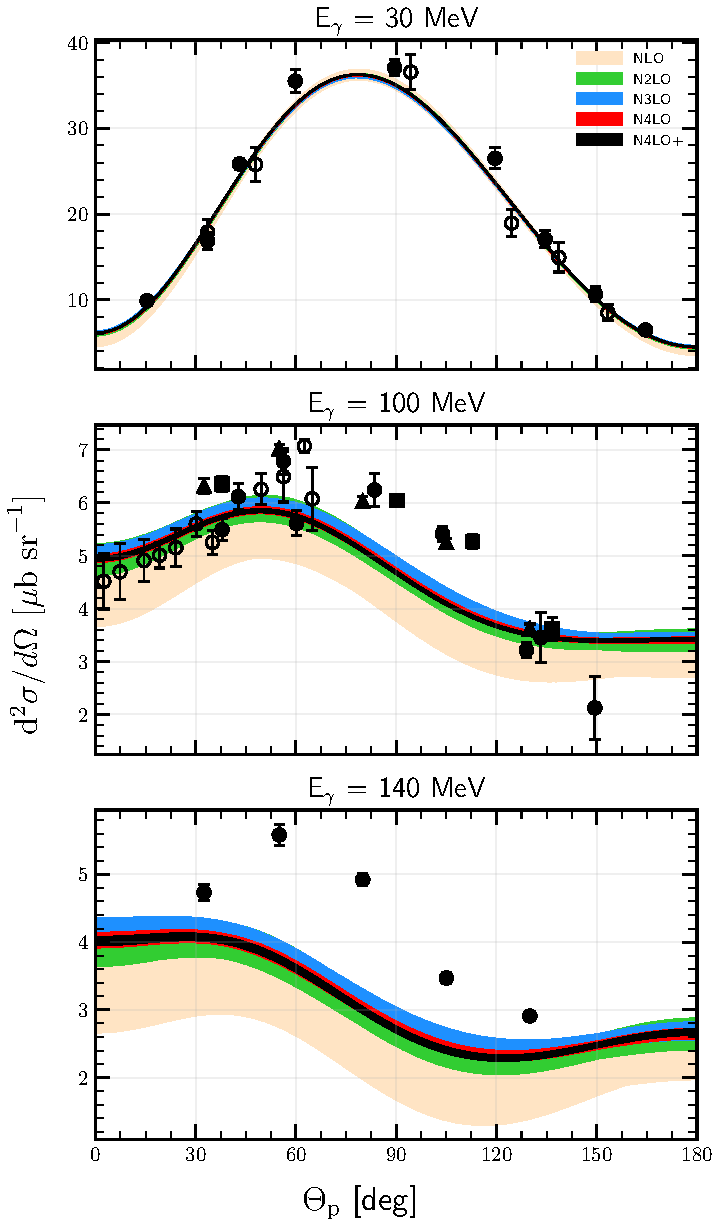
\includegraphics[width=0.7\textwidth]{Figures_python/CROSS2_truncation_vert.pdf}
        \end{center}
        \caption{Truncation error's bands for the differential cross section 
        as a function of the outgoing proton angle in the center of mass frame 
        The photon's energy is 30 MeV (top pane), 100 MeV (middle) and 140 MeV (bottom). Results are obtained using potential
        with different chiral orders (from LO to N$^4$LO+) with cutoff parameter $\Lambda=450$~MeV.
        Data points (filled and empty circles) are from \cite{Ying_Experiment_Deut}
        for (30 and 100 meV)
        and \cite{DeSanctis_Experiment_Deut} (for energy 140 MeV).}
        \label{Diff_cross_truncation}
    \end{figure}

    

    \begin{figure}[h]
        \begin{center}
        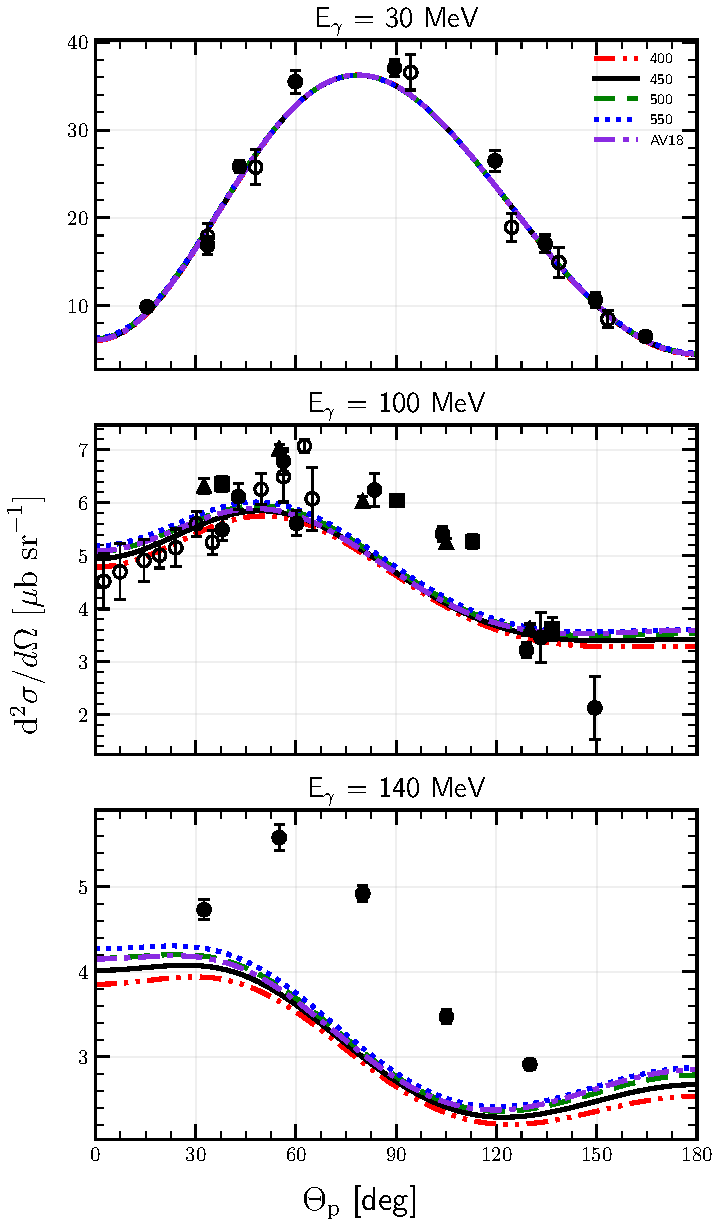
\includegraphics[width=0.7\textwidth]{Figures_python/CROSS2_cutoff_vert.pdf}
        \end{center}
        \caption{Truncation error's bands for the differential cross section 
        as a function of the outgoing proton angle in the center of mass frame 
        ThDifferential cross section as a function of the outgoing proton angle in the center of mass frame 
        for the photon's energy is 30 MeV (top pane), 100 MeV (middle) and 140 MeV (bottom). 
        The double-dotted-dashed red line presents results obtaining with 
        a cutoff values $\Lambda=400$~MeV, solid black line - 450~MeV, dashed green line - 500~MeV
    and dotted blues line - 550~MeV.
        For the sake of comparison, predictions obtained with AV18 potential (purple dotted-dashed line).
        Data points (filled and empty circles) are from \cite{Ying_Experiment_Deut}
        for (30 and 100 meV)
        and \cite{DeSanctis_Experiment_Deut} (for energy 140 MeV).}
        \label{Diff_cross_cutoff}
    \end{figure}

    
        
    % \begin{figure}[h]
    %     \begin{center}
    %     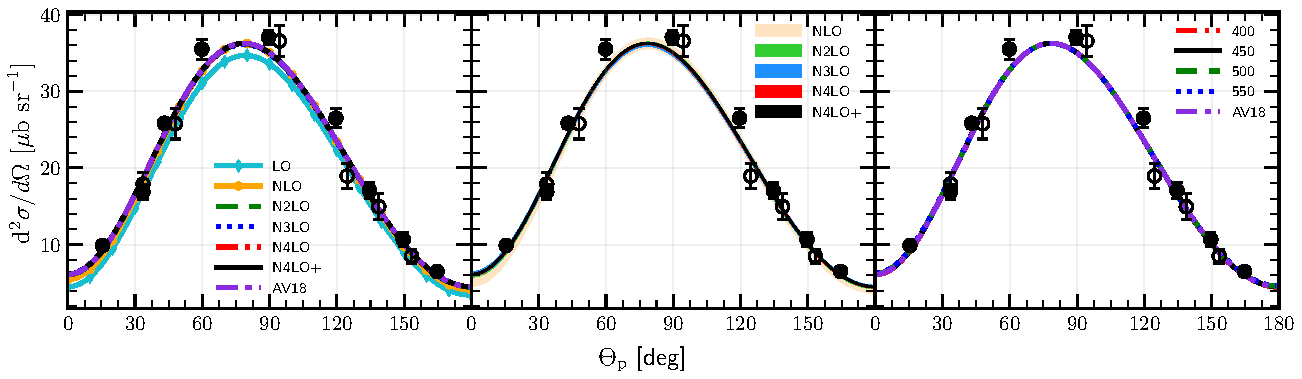
\includegraphics[width=0.95\textwidth]{Figures_python/CROSS2_30mev.pdf}
    %     \end{center}
    %     \caption{Differential cross section as a function of the outgoing proton angle in the center of mass frame 
    %     for the photon's energy 30 MeV. Left figure presents results obtained using potential
    %     with different chiral orders (from LO to N$^4$LO+) with cutoff parameter $\Lambda=450$~MeV
    %     whereas right figure presents a cutoff dependency and chiral potential N$^4$LO+ was used in all cases.
    %     For the sake of comparison, predictions obtained with AV18 potential are on both figures as well.
    %     Data points (filled and empty circles) are from \cite{Ying_Experiment_Deut}.}
    %     \label{CROSS_30}
    % \end{figure}
        

    % \begin{figure}[h]
    %     \begin{center}
    %     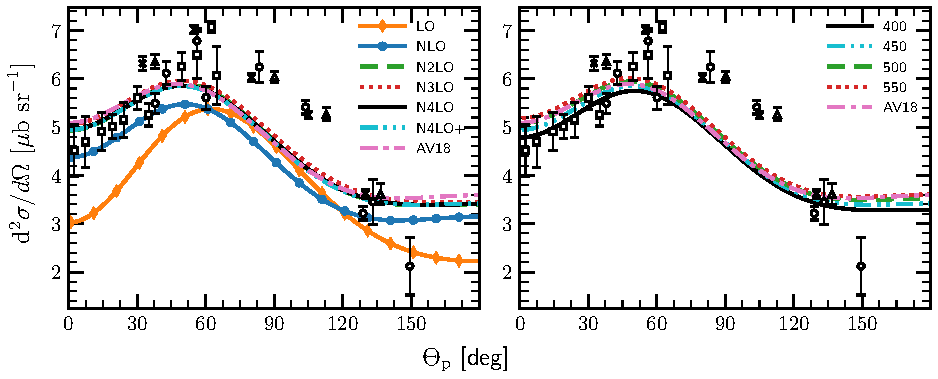
\includegraphics[width=0.95\textwidth]{Figures_python/CROSS2_100mev.pdf}
    %     \end{center}
    %     \caption{The same as on the Fig.~\ref{CROSS_30} but for the photon's energy E$_\gamma$=100~MeV.
    %     All experimental data points (filled and empty circles, squares and triangles) are from \cite{Ying_Experiment_Deut}.}
    %     \label{CROSS_100}
    % \end{figure}

    % \begin{figure}[h]
    %     \begin{center}
    %     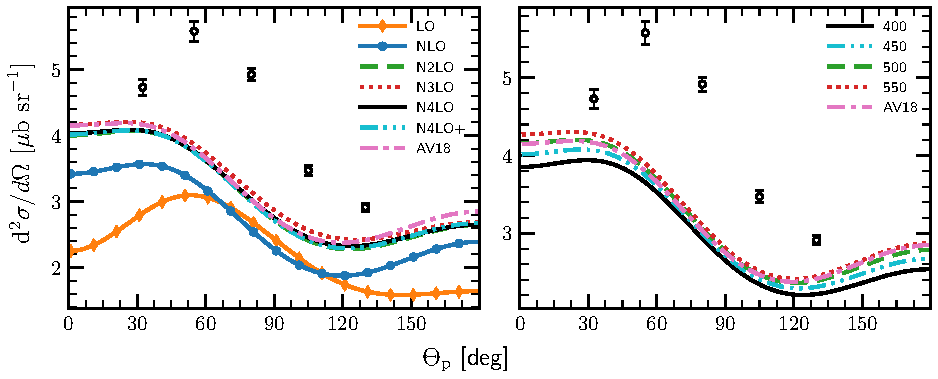
\includegraphics[width=0.95\textwidth]{Figures_python/CROSS2_140mev.pdf}
    %     \end{center}
    %     \caption{The same as on the Fig.~\ref{CROSS_30} but for the photon's energy E$_\gamma$=140~MeV.
    %     The data are from \cite{DeSanctis_Experiment_Deut}.}
    %     \label{CROSS_140}
    % \end{figure}
        
    \subsection{Tensor analyzing power}

      

    \begin{figure}[h]
        \begin{center}
        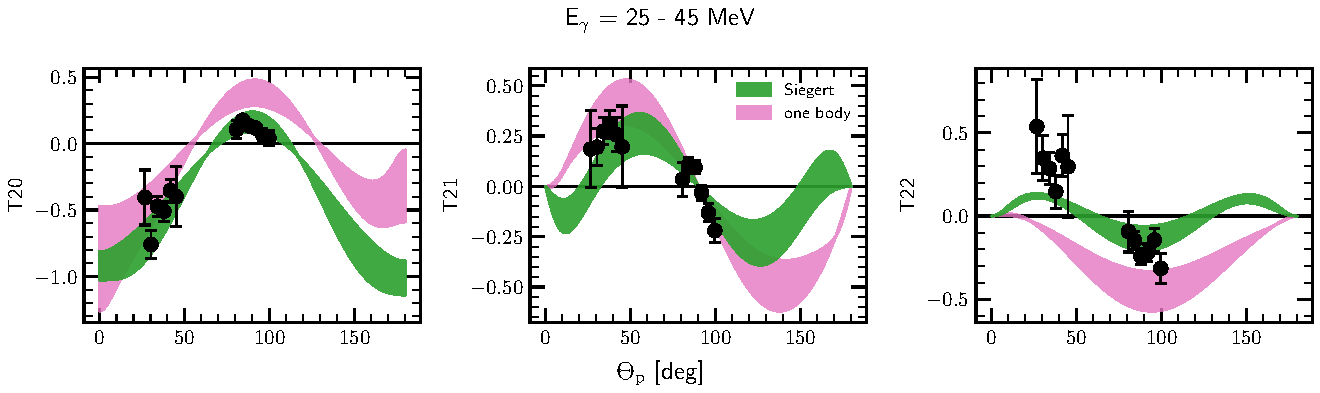
\includegraphics[width=1\textwidth]{Figures_python/Tensor_analyzing_power_angular_E25-45.pdf}
        \end{center}
        \caption{Tensor analyzing powers T$_{20}$, T$_{21}$ and T$_{22}$ as a functions of the
        outgoing proton angle $\theta_p$ (in the center of mass frame).
        Solid blue line is a mean value of my predictions obtained with a
        SMS potential at N$^4$LO+ chiral order and with $\Lambda$~=~450~MeV
        at energy values from 25 to 45 MeV and
        where SN current was used together with Siegert approach. 
        Pink dashed line is similar prediction but with SN only. 
        The corresponding bands show the deviation of predictions in the regarded
        energy region.
        % Filled bands show maximal spread of my predictions obtained with a 
        % SMS potential at N$^4$LO+ chiral order and with $\Lambda$~=~450~MeV
        % for the energy span from 25 to 45 MeV. Blue bands correspond to the
        % case where SN current was used together with Siegert approach and 
        % pink bands - to the SN currentonly. 
        Filled circles are experimental data
        from \cite{rachek2007} for the analogous energy span.}
        \label{tensor_angular_25-45}
    \end{figure}

    \begin{figure}[h]
        \begin{center}
        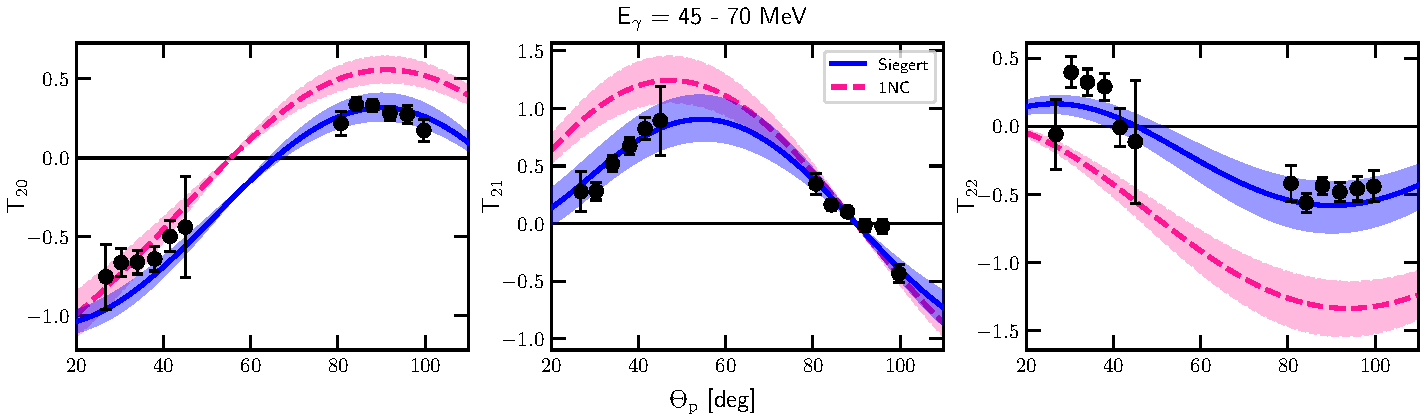
\includegraphics[width=0.95\textwidth]{Figures_python/Tensor_analyzing_power_angular_E45-70.pdf}
        \end{center}
        \caption{The same as on the Fig.~\ref*{tensor_angular_25-45} but for energy bin 45~-~70~MeV}
        \label{tensor_angular_45-70}
    \end{figure}

    \begin{figure}[h]
        \begin{center}
        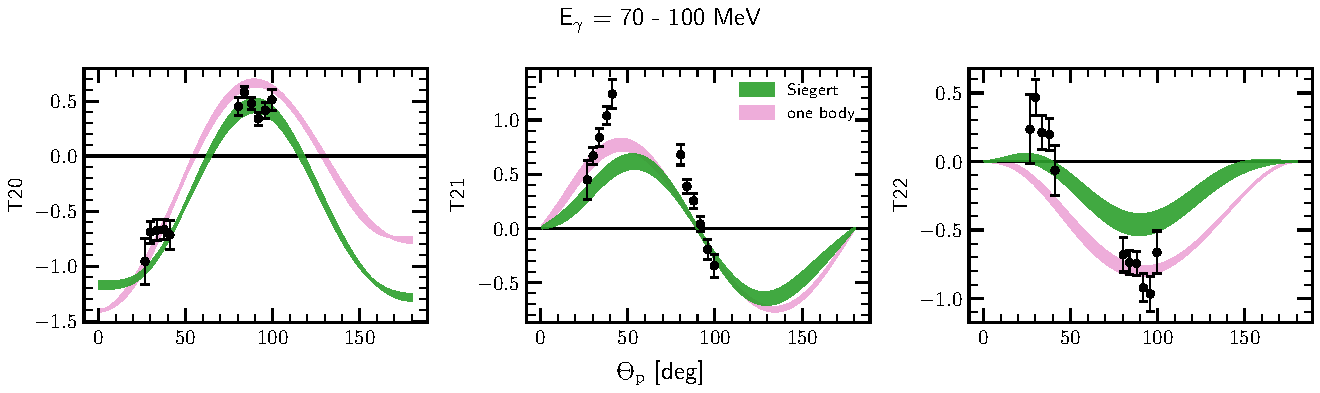
\includegraphics[width=0.95\textwidth]{Figures_python/Tensor_analyzing_power_angular_E70-100.pdf}
        \end{center}
        \caption{The same as on the Fig.~\ref*{tensor_angular_25-45} but for energy bin 70~-~100~MeV}
        \label{tensor_angular_70-100}
    \end{figure}        

    \begin{figure}[h]
        \begin{center}
        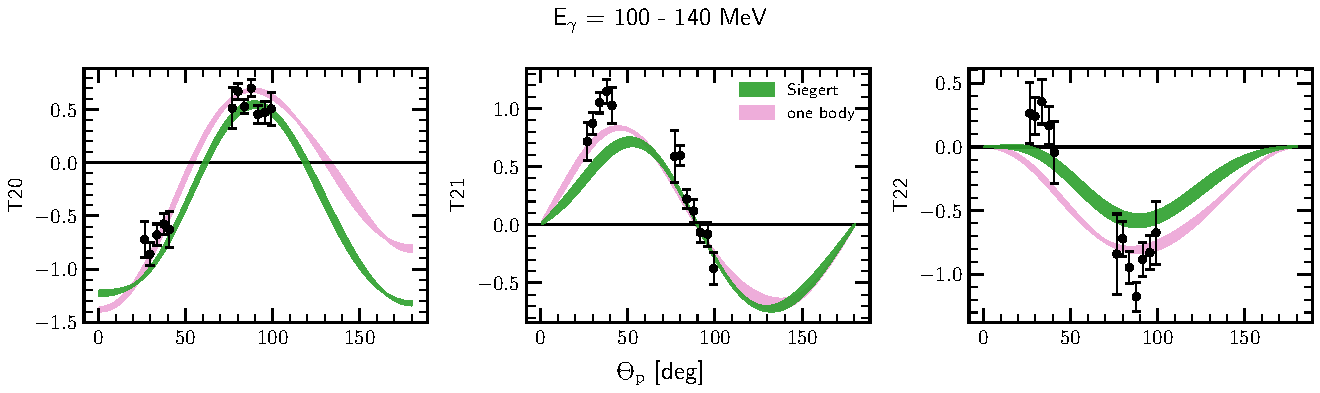
\includegraphics[width=0.95\textwidth]{Figures_python/Tensor_analyzing_power_angular_E100-140.pdf}
        \end{center}
        \caption{The same as on the Fig.~\ref*{tensor_angular_25-45} but for energy bin 100~-~140~MeV}
        \label{tensor_angular_100-140}
    \end{figure}
        
        

    \begin{figure}[h]
        \begin{center}
        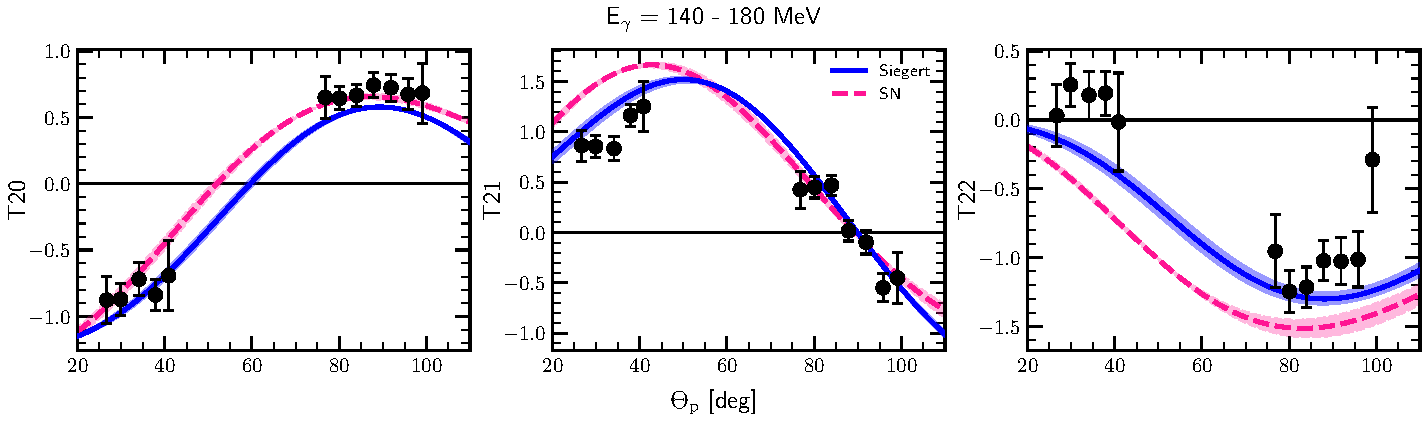
\includegraphics[width=0.95\textwidth]{Figures_python/Tensor_analyzing_power_angular_E140-180.pdf}
        \end{center}
        \caption{The same as on the Fig.~\ref*{tensor_angular_25-45} but for energy bin 140~-~180~MeV}
        \label{tensor_angular_140-180}
    \end{figure}
        

    \begin{figure}[h]
        \begin{center}
        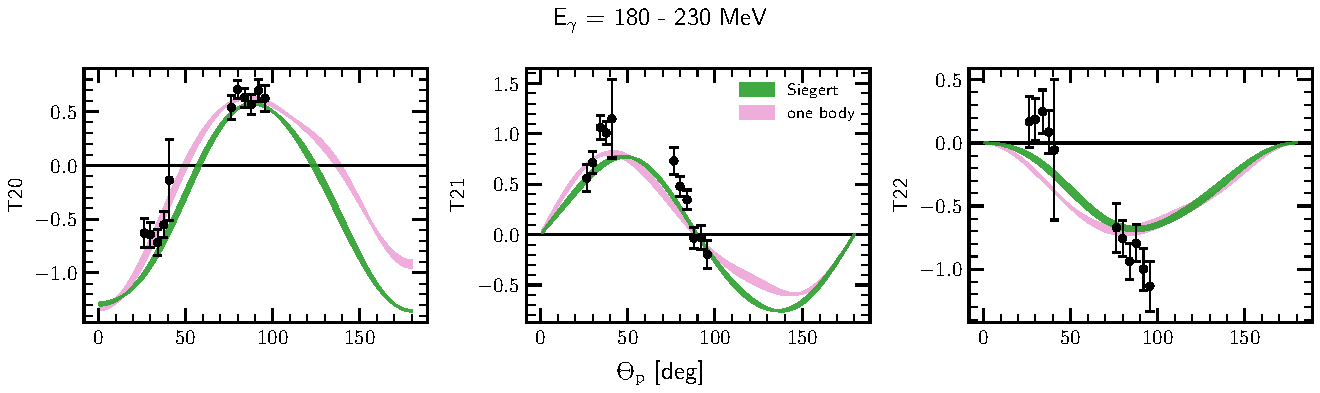
\includegraphics[width=0.95\textwidth]{Figures_python/Tensor_analyzing_power_angular_E180-230.pdf}
        \end{center}
        \caption{The same as on the Fig.~\ref*{tensor_angular_25-45} but for energy bin 180~-~230~MeV}
        \label{tensor_angular_180-230}
    \end{figure}

    \begin{figure}[h]
        \begin{center}
        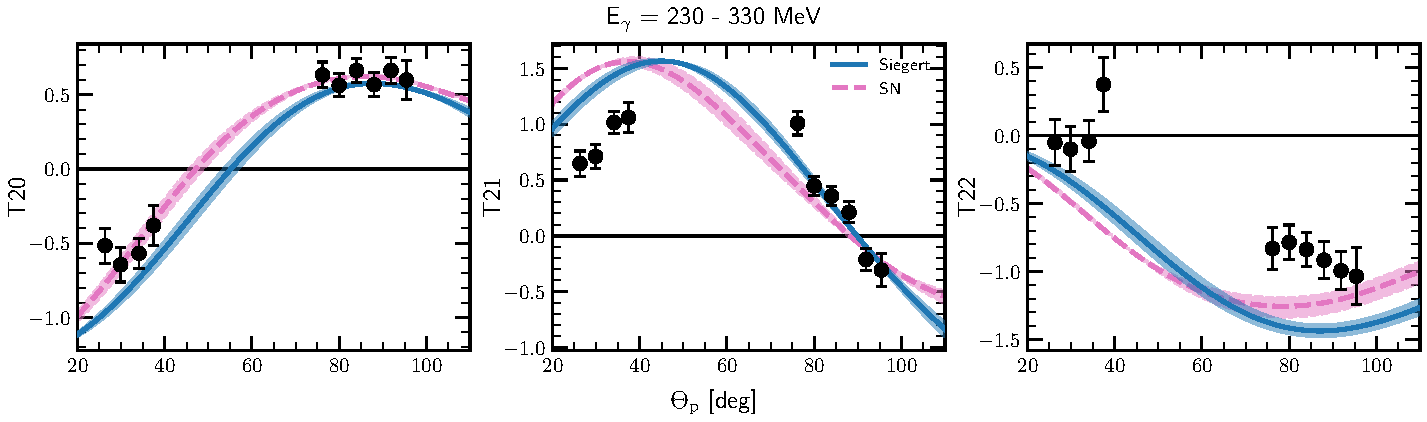
\includegraphics[width=0.95\textwidth]{Figures_python/Tensor_analyzing_power_angular_E230-330.pdf}
        \end{center}
        \caption{The same as on the Fig.~\ref*{tensor_angular_25-45} but for energy bin 230~-~330~MeV}
        \label{tensor_angular_230-330}
    \end{figure}
        


    \begin{figure}[h]
        \begin{center}
        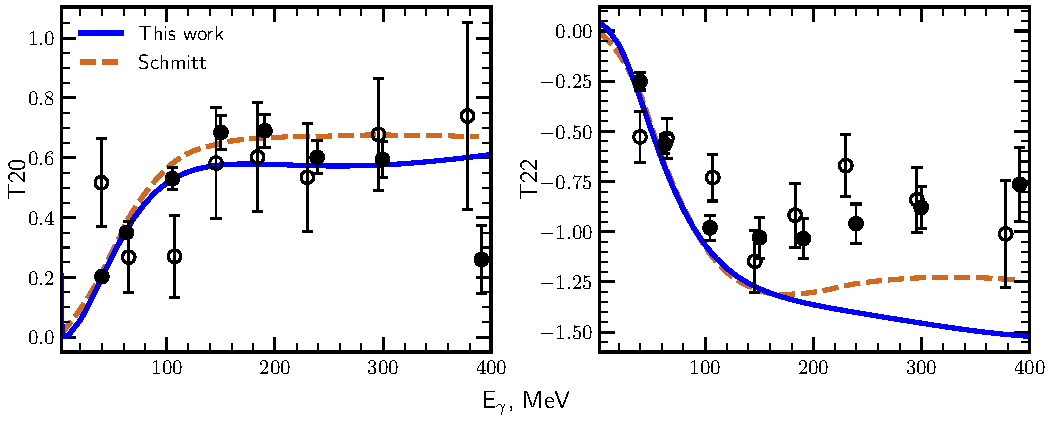
\includegraphics[width=0.75\textwidth]{Figures_python/T20_T22_vs_en.pdf}
        \end{center}
        \caption{Tensor analyzing powers T$_{20}$ and T$_{22}$ as a functions of the photon energy E$_\gamma$
        with fixed outgoing proton angle $\theta_p = 88^{\circ}$ (in the center of mass frame).
        My predictions (blue solid line) are obtained with SMS potential at chiral order N$^4$LO+
        and with cutoff parameter $\Lambda$~=~450~MeV.
        Dashed brown line presents calculations from \cite{Schmitt1989}.
        Experimental data is taken from \cite{rachek2007} (filled circles)
        and \cite{mishev1993} (empty circles).}
        \label{T20_vs_en}
    \end{figure}

    \begin{figure}[h]
        \begin{center}
        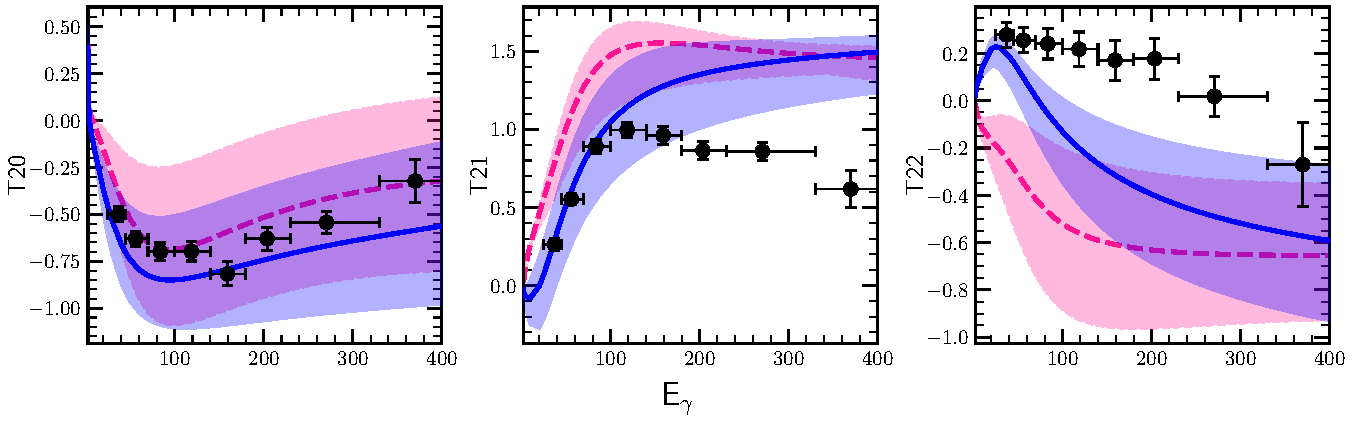
\includegraphics[width=0.95\textwidth]{Figures_python/TensorPower_Th24-48.pdf}
        \end{center}
        \caption{Tensor analyzing powers T$_{20}$, T$_{21}$ and T$_{22}$ as a functions of the
        photon's energy within the outgoing proton's angle range $24^{\circ} - 48^{\circ}$
        (in the center of mass frame).
        Solid blue line is a mean value of my predictions obtained with
        SMS potential at N$^4$LO+ chiral order and with $\Lambda$~=~450~MeV
        at energy values from 25 to 45 MeV within
        a given angles range and
        where SN current was used together with Siegert approach. 
        Pink dashed line is similar prediction but with SN only. 
        The corresponding bands show the deviation of predictions in the regarded
        energy region.
        Filled circles are experimental data
        from \cite{rachek2007} for the analogous energy span.}
        \label{tensor_energy_24-48}
    \end{figure}

    \begin{figure}[h]
        \begin{center}
        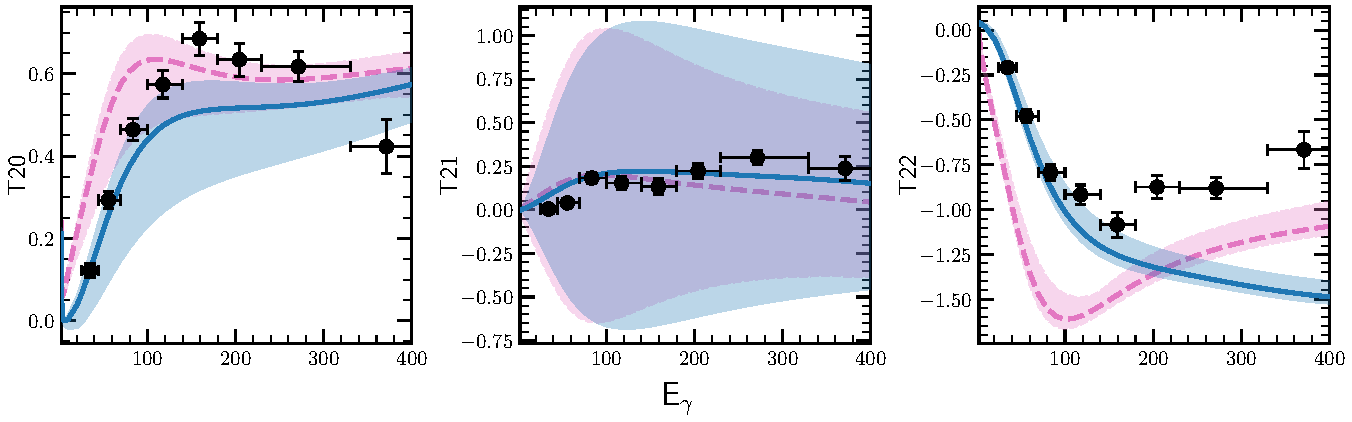
\includegraphics[width=0.95\textwidth]{Figures_python/TensorPower_Th70-102.pdf}
        \end{center}
        \caption{The same as on the Fig.~\ref*{tensor_energy_24-48} but
        for the angles' range $70^{\circ} - 102^{\circ}$.}
        \label{tensor_energy_70-102}
    \end{figure}
        
    % I will try to figure out why we can see such a wide band of predictions
    % for $T_{20}$ in the Fig.~\ref*{tensor_energy_24-48} and
    % for $T_{21}$  in the Fig.~\ref*{tensor_energy_70-102}.
    % Let's stick to the particular energy value E$_\gamma = 120$~MeV.
    % The spread of predictions is high in the both cases for such energy value.
    % The corresponding angular distribution of these observables
    % one can find on the  Fig.~\ref*{tensor_angular_100-140}
    % (of course there is some energy range on the Figure, but let's assume that 
    % energy dependance is not so strong around 120~MeV and for $T_{20}$
    % it is confirmed by the Fig.~\ref*{T20_vs_en}).
    % In the first case we have a prediction for angles' range $24^{\circ} - 48^{\circ}$
    % and we can see that $T_{20}$ in this region has 